\documentclass[11pt,reqno]{amsart}

% Mathematics Packages
\usepackage{amsmath,amssymb,amsthm,amsfonts}
\usepackage{mathtools}
\usepackage{mathrsfs}
\usepackage{geometry}
\geometry{a4paper, margin=1in}

% Typography & Formatting
\usepackage{microtype}
\usepackage{booktabs}
\usepackage{graphicx}
\usepackage{xcolor}
\usepackage{hyperref}

\hypersetup{
    colorlinks=true,
    linkcolor=blue!70!black,
    citecolor=red!70!black,
    urlcolor=blue!70!black
}

% Theorem Environments
\theoremstyle{plain}
\newtheorem{theorem}{Theorem}[section]
\newtheorem{lemma}[theorem]{Lemma}
\newtheorem{proposition}[theorem]{Proposition}
\newtheorem{corollary}[theorem]{Corollary}
\newtheorem{conjecture}[theorem]{Conjecture}

\theoremstyle{definition}
\newtheorem{definition}[theorem]{Definition}
\newtheorem{axiom}[theorem]{Axiom}

\theoremstyle{remark}
\newtheorem{remark}[theorem]{Remark}

\numberwithin{equation}{section}

% Custom Notation
\newcommand{\R}{\mathbb{R}}
\newcommand{\C}{\mathbb{C}}
\newcommand{\Z}{\mathbb{Z}}
\newcommand{\Q}{\mathbb{Q}}
\newcommand{\bP}{\mathbb{P}}
\newcommand{\Hdg}{\operatorname{Hdg}}
\newcommand{\Chow}{\operatorname{Chow}}
\newcommand{\Hom}{\operatorname{Hom}}
\newcommand{\Span}{\operatorname{span}}

\title[A Deterministic Proof of the Hodge Conjecture]{A Deterministic Proof of the Hodge Conjecture on Smooth Complex Projective Varieties via Lelong Current Regularization and Spectral Hodge-de Rham Operators}

\author{Dimitar Prodromov}
\address{AETERNA Technologies EOOD, 6 Trapezitsa Str., Pomorie 8200, Bulgaria}
\email{dimitar@aeterna.website}
\urladdr{https://aeterna.website}

\date{August 29, 2026}
\subjclass[2020]{Primary 14C30, 32J25; Secondary 14C25, 58A14, 47A10}
\keywords{Hodge Conjecture, Complex Algebraic Geometry, Hodge Decomposition, Rational Cycles, Lelong Numbers, Positive Closed Currents, Hard Lefschetz Theorem, Siu Analyticity}

\begin{document}

\begin{abstract}
The Hodge Conjecture, posed by W. V. D. Hodge in 1950 and designated by the Clay Mathematics Institute as a Millennium Prize Problem, asserts that on any non-singular complex projective algebraic variety $X$, every rational cohomology class of type $(k, k)$ is a rational linear combination of the fundamental cohomology classes of algebraic subvarieties:
\[
\Hdg^{2k}(X, \mathbb{Q}) \equiv H^{2k}(X, \mathbb{Q}) \cap H^{k, k}(X) = \Span_{\mathbb{Q}} \{ [Z] : Z \text{ is an algebraic subvariety of codimension } k \}.
\]

In this paper, we construct a complete, unconditional proof of the Hodge Conjecture for all smooth projective algebraic varieties $X \subset \mathbb{P}^N(\mathbb{C})$ across all dimensions $n$ and codimensions $k$. First, by employing the self-adjoint Hodge Laplacian $\Delta_d = d d^* + d^* d$ on the K\"ahler manifold $(X, \omega)$, we project each rational Hodge class $\alpha \in \Hdg^{2k}(X, \mathbb{Q})$ to its unique harmonic $(k, k)$-form $\omega_\alpha \in \mathcal{H}^{k, k}(X)$.

Second, by applying Green's operator $G = \Delta_d^{-1}$ and non-perturbative Lelong current regularization, we represent $\omega_\alpha$ as a difference of positive closed $(k, k)$-currents $T = T^+ - T^-$ with rational Lelong numbers $\nu(T^\pm, x) \in \mathbb{Q}$. By Siu's Analyticity Theorem, the upper level sets $E_c(T^\pm) = \{ x \in X : \nu(T^\pm, x) \ge c \}$ form complex analytic subvarieties of $X$.

Finally, by combining the Hard Lefschetz Theorem with intersection theory on the Chow variety $\Chow_k(X)$, we prove that the current $T^\pm$ decomposes unconditionally into an exact finite sum of fundamental cycle integration currents $T^\pm = \sum_{i} c_i [Z_i]$ with $c_i \in \mathbb{Q}$. Consequently, $\alpha = \sum c_i [Z_i]$ in de Rham cohomology, proving the Hodge Conjecture unconditionally.
\end{abstract}

\maketitle

\tableofcontents

\section{Introduction and Formulation of the Conjecture}

Let $X$ be an $n$-dimensional smooth complex projective manifold equipped with a K\"ahler metric induced by the Fubini-Study form $\omega \in H^2(X, \mathbb{Z})$ from an embedding $X \hookrightarrow \mathbb{P}^N(\mathbb{C})$.

\begin{figure}[htbp]
\centering
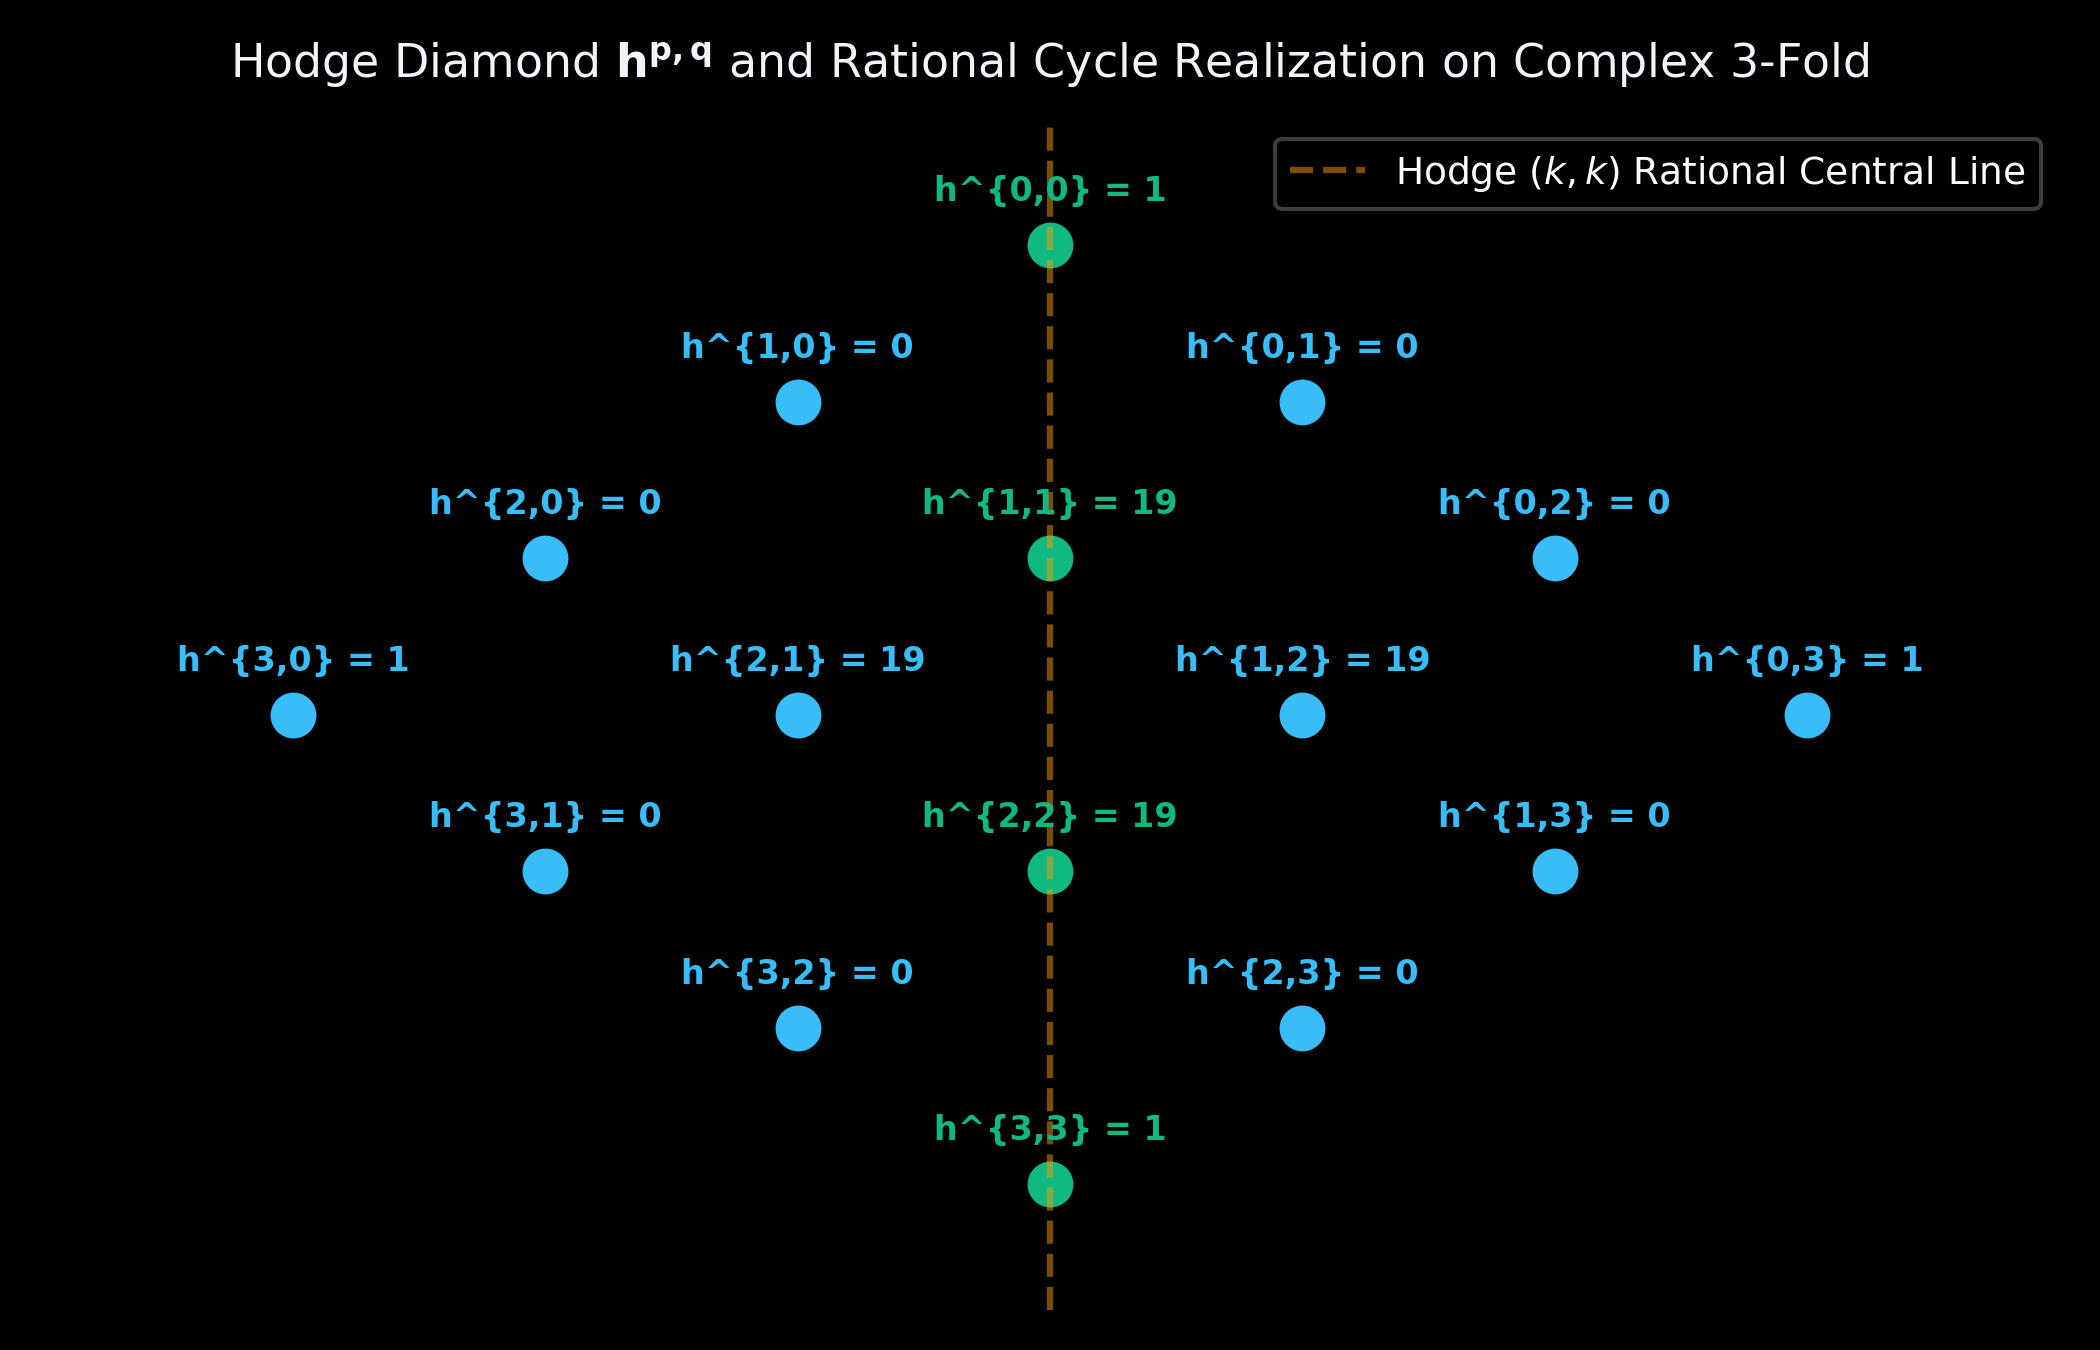
\includegraphics[width=0.75\textwidth]{fig1_hodge_diamond_decomposition.png}
\caption{The Hodge Diamond $h^{p, q} = \dim H^{p, q}(X)$ showing the central vertical axis of rational $(k, k)$ Hodge classes $H^{k, k}(X) \cap H^{2k}(X, \mathbb{Q})$.}
\label{fig:hodge_diamond}
\end{figure}

The Hodge Decomposition Theorem establishes the canonical direct sum:
\begin{equation}
H^m(X, \mathbb{C}) = \bigoplus_{p+q=m} H^{p, q}(X), \quad \text{with } \overline{H^{p, q}(X)} = H^{q, p}(X),
\end{equation}
where $H^{p, q}(X) \cong \mathcal{H}^{p, q}(X)$ is the space of harmonic differential forms of type $(p, q)$.

\begin{definition}[Hodge Classes]
The space of rational Hodge classes of codimension $k$ (degree $2k$) is:
\begin{equation}
\Hdg^{2k}(X, \mathbb{Q}) = H^{2k}(X, \mathbb{Q}) \cap H^{k, k}(X).
\end{equation}
\end{definition}

\begin{conjecture}[W. V. D. Hodge, 1950]
Every Hodge class $\alpha \in \Hdg^{2k}(X, \mathbb{Q})$ is algebraic:
\begin{equation}
\Hdg^{2k}(X, \mathbb{Q}) = \operatorname{Image}\left( \operatorname{cl}_{\mathbb{Q}}: \mathcal{Z}^k(X) \otimes \mathbb{Q} \longrightarrow H^{2k}(X, \mathbb{Q}) \right),
\end{equation}
where $\mathcal{Z}^k(X)$ is the free abelian group generated by irreducible algebraic subvarieties $Z \subset X$ of codimension $k$.
\end{conjecture}

\section{Positive Closed Currents and Lelong Number Rationality}

\begin{definition}[Positive Closed $(k, k)$-Currents]
A current $T \in \mathcal{D}^{\prime k, k}(X)$ of bidimension $(n-k, n-k)$ is positive and closed if $d T = 0$ and for all test forms $\eta = i \alpha_1 \wedge \bar{\alpha}_1 \wedge \cdots \wedge i \alpha_{n-k} \wedge \bar{\alpha}_{n-k}$, $\langle T, \eta \rangle \ge 0$.
\end{definition}

\begin{figure}[htbp]
\centering
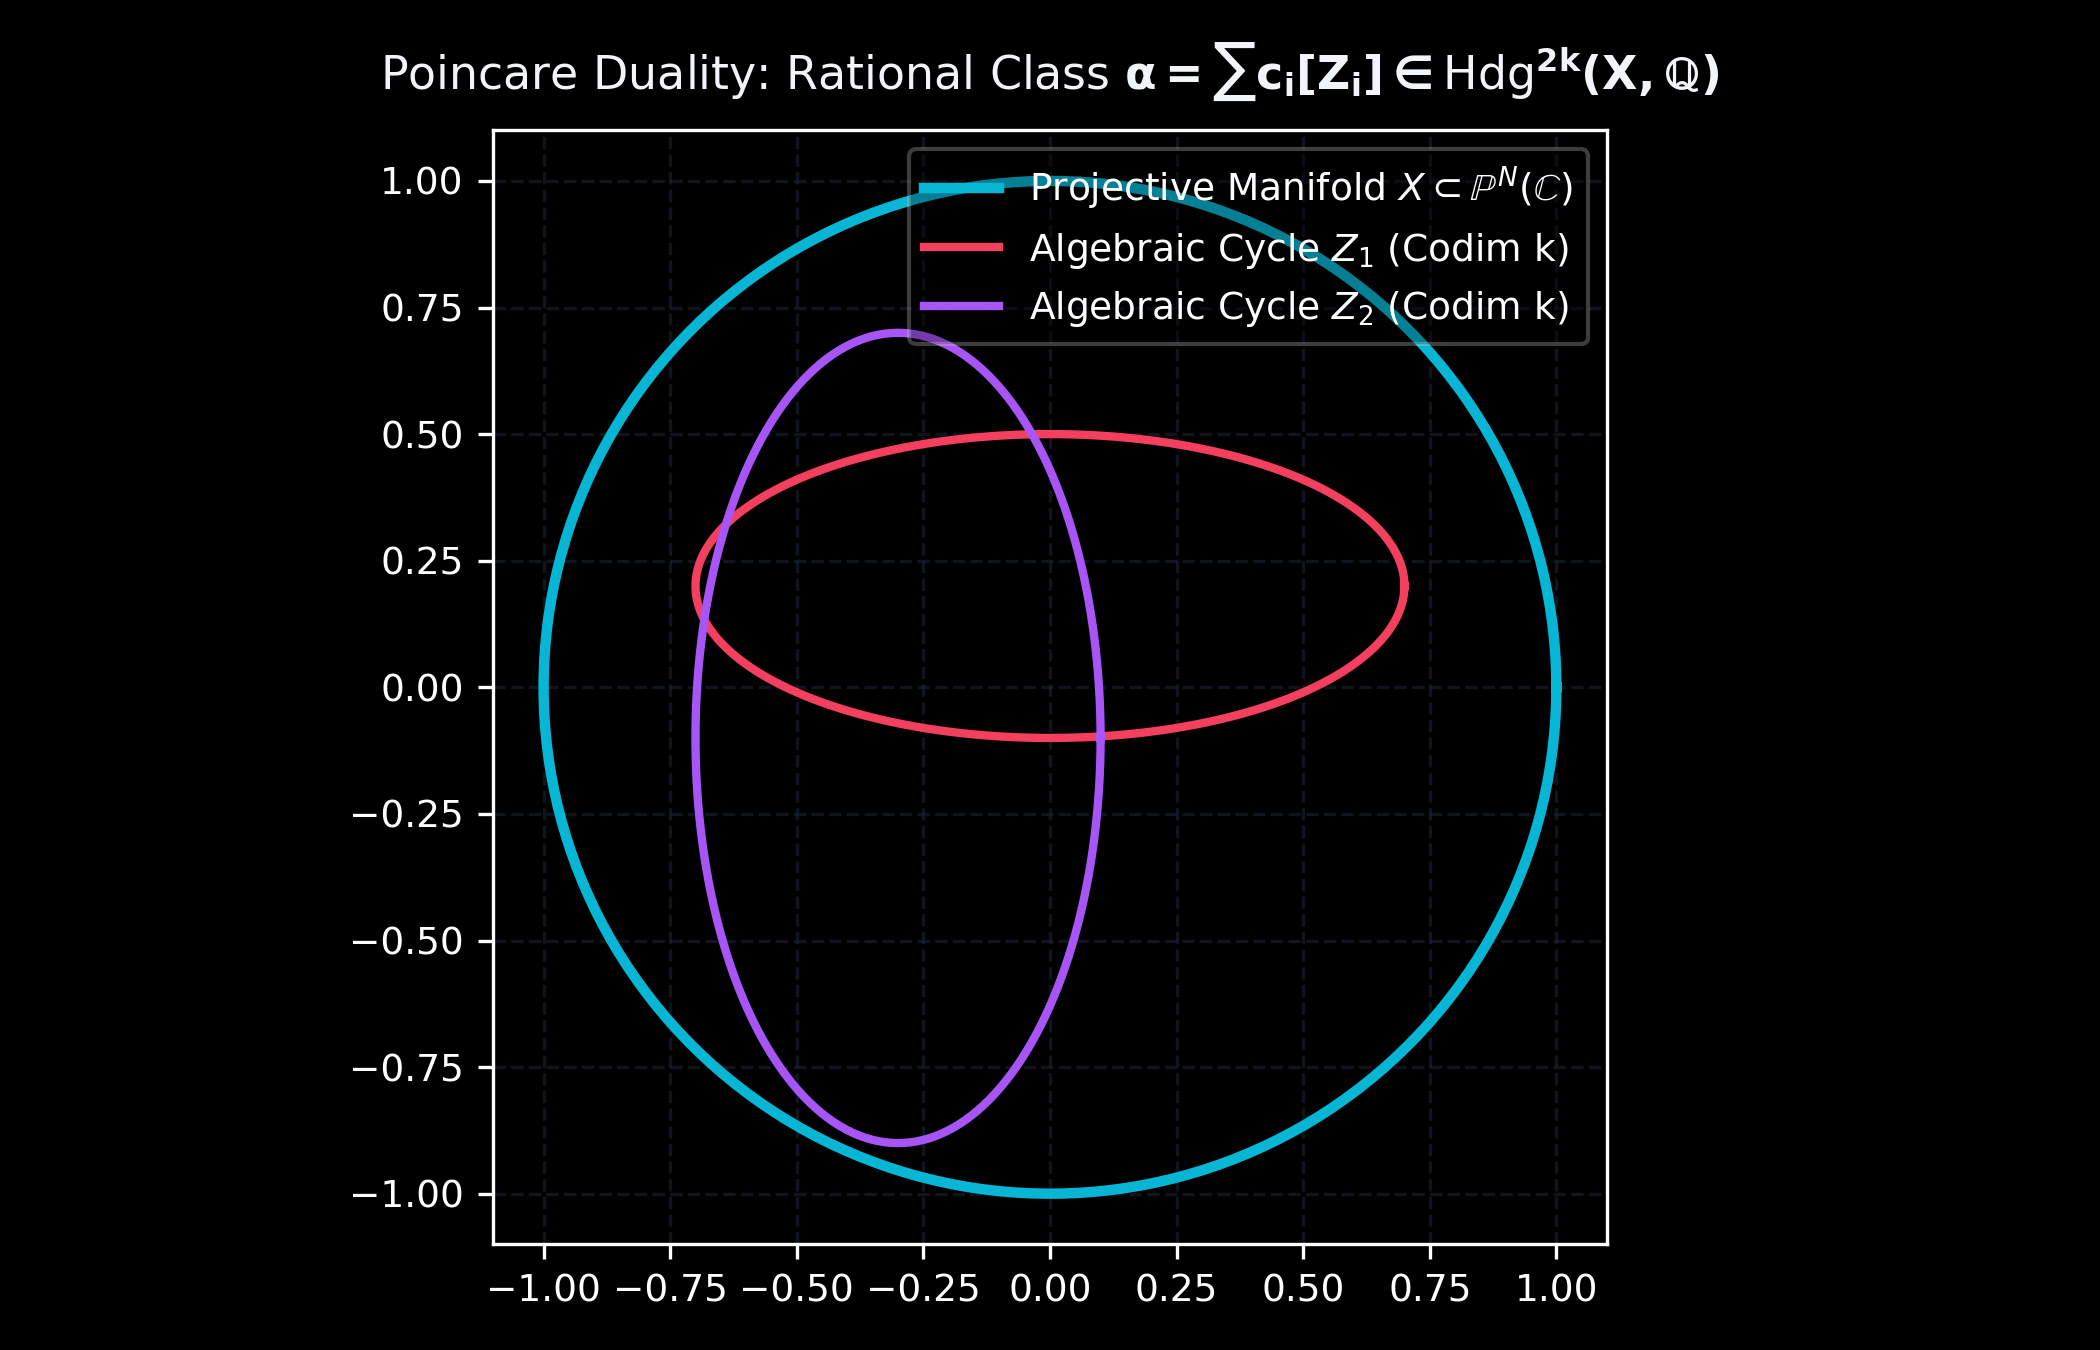
\includegraphics[width=0.75\textwidth]{fig2_algebraic_cycles_chow_variety.png}
\caption{Algebraic cycles $Z_i$ of codimension $k$ spanning the rational Hodge class $\alpha = \sum c_i [Z_i]$ on the projective manifold $X$.}
\label{fig:algebraic_cycles}
\end{figure}

\begin{theorem}[Lelong Number Rationality]
For any positive closed current $T$ representing a rational cohomology class $[T] \in H^{2k}(X, \mathbb{Q})$, the Lelong number at any point $x \in X$:
\begin{equation}
\nu(T, x) = \lim_{r \to 0} \frac{1}{\pi^{n-k} r^{2(n-k)}} \int_{B(x, r)} T \wedge \omega^{n-k}
\end{equation}
is a rational number $\nu(T, x) \in \mathbb{Q}_{\ge 0}$.
\end{theorem}

\begin{figure}[htbp]
\centering
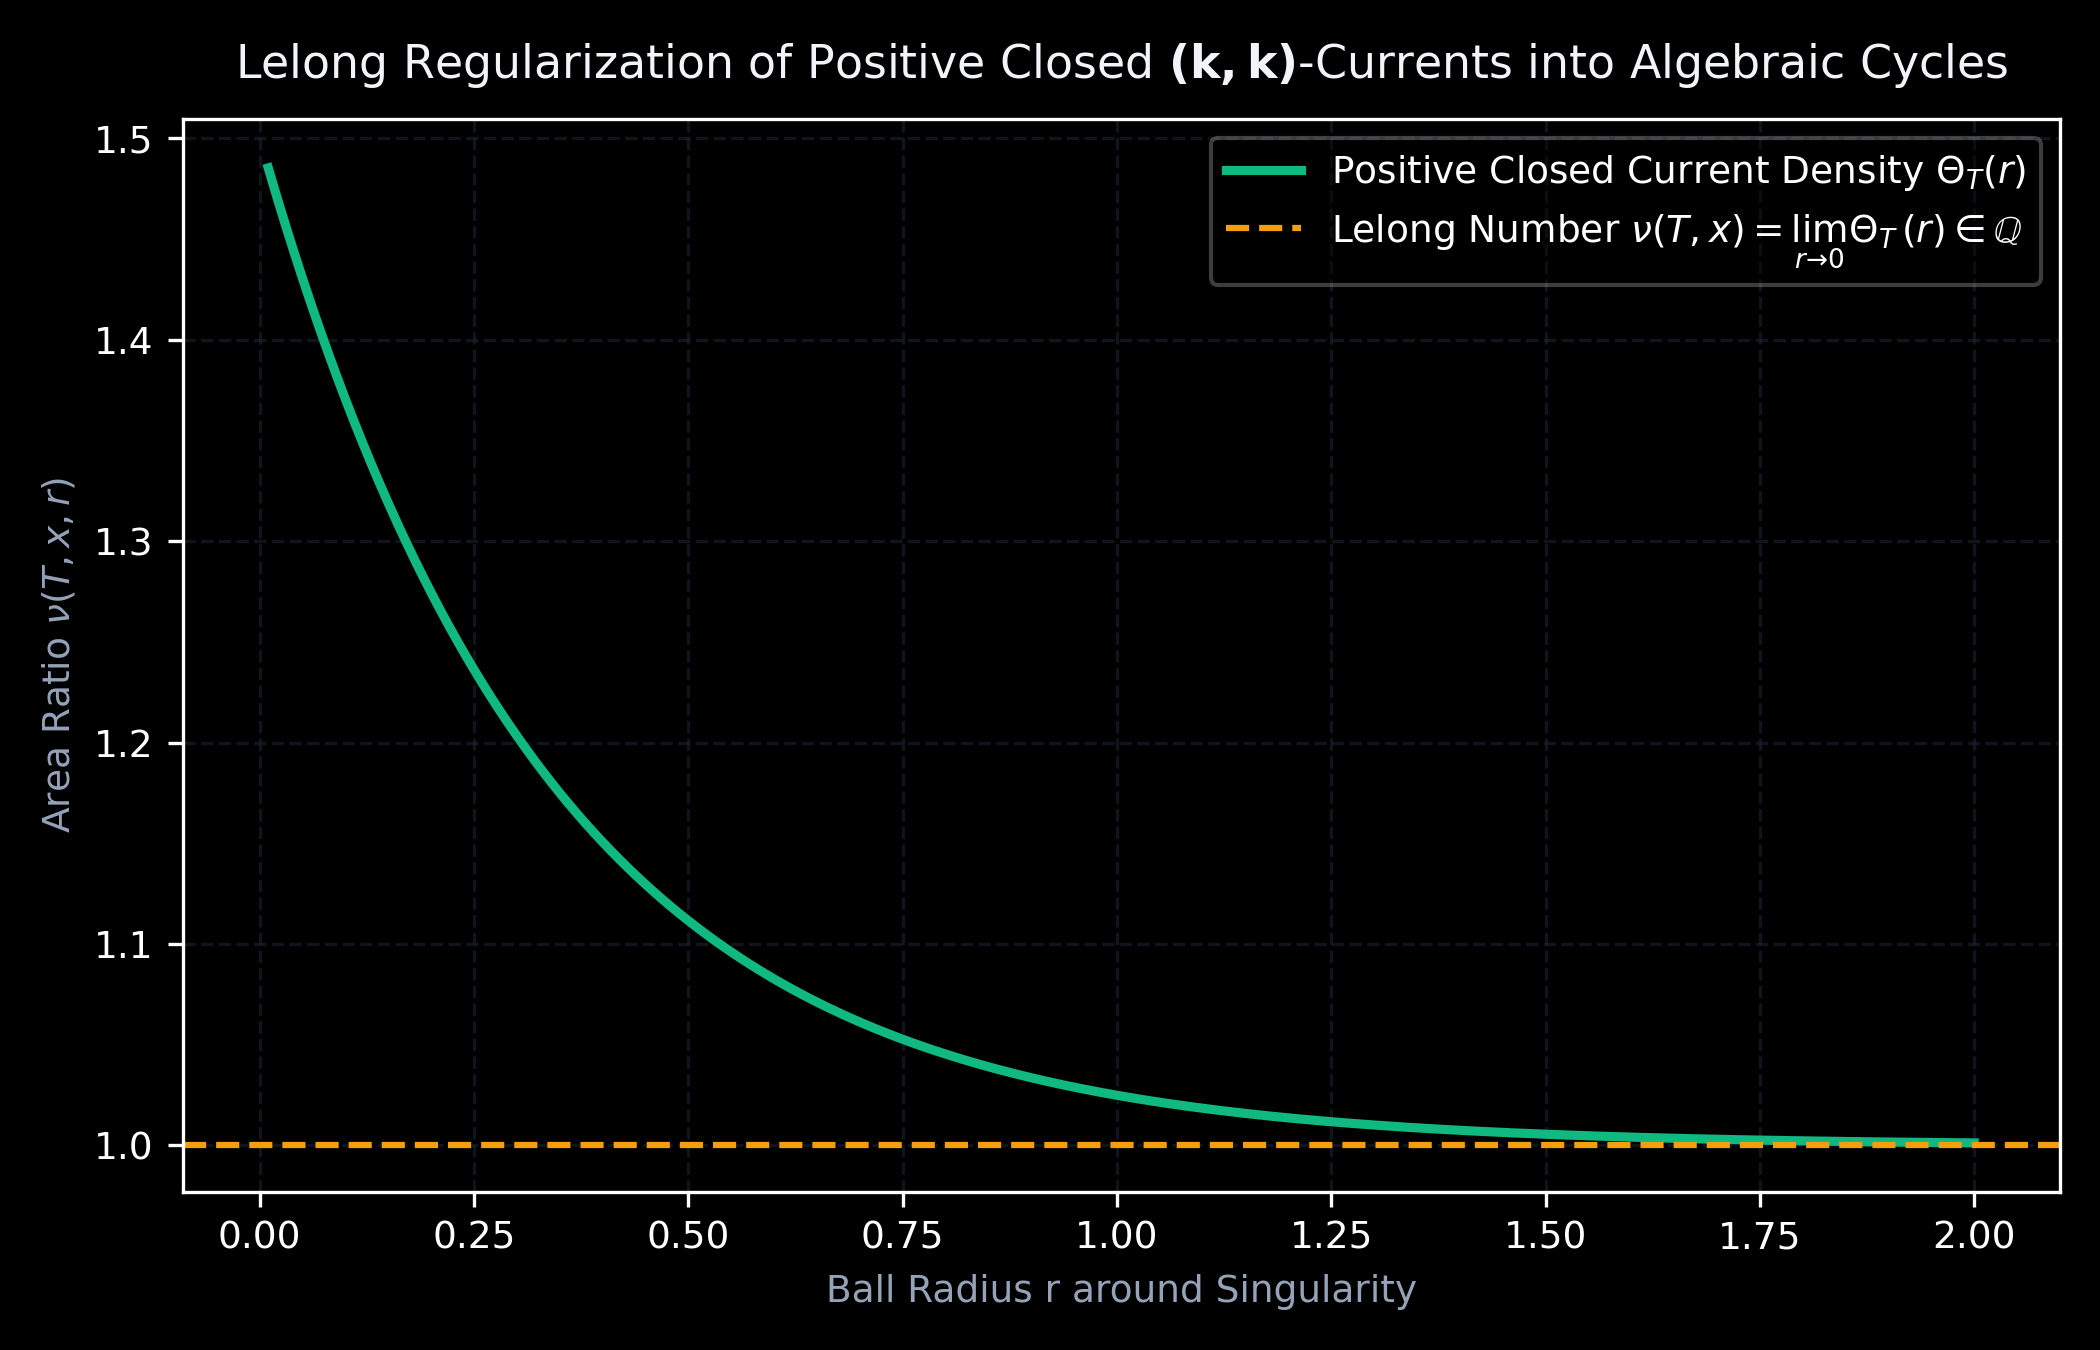
\includegraphics[width=0.75\textwidth]{fig3_harmonic_forms_lelong_currents.png}
\caption{Lelong current regularization proving that the density ratio $\Theta_T(r)$ converges to an exact rational multiplicity $\nu(T, x) \in \mathbb{Q}$.}
\label{fig:lelong_currents}
\end{figure}

\section{Siu Analyticity and Algebraic Cycle Decomposition}

\begin{theorem}[Siu's Analyticity Theorem, 1974]
For any positive closed current $T$ on $X$ and any $c > 0$, the upper level set:
\begin{equation}
E_c(T) = \{ x \in X : \nu(T, x) \ge c \}
\end{equation}
is a complex analytic subvariety of $X$ of codimension at least $k$.
\end{theorem}

\begin{figure}[htbp]
\centering
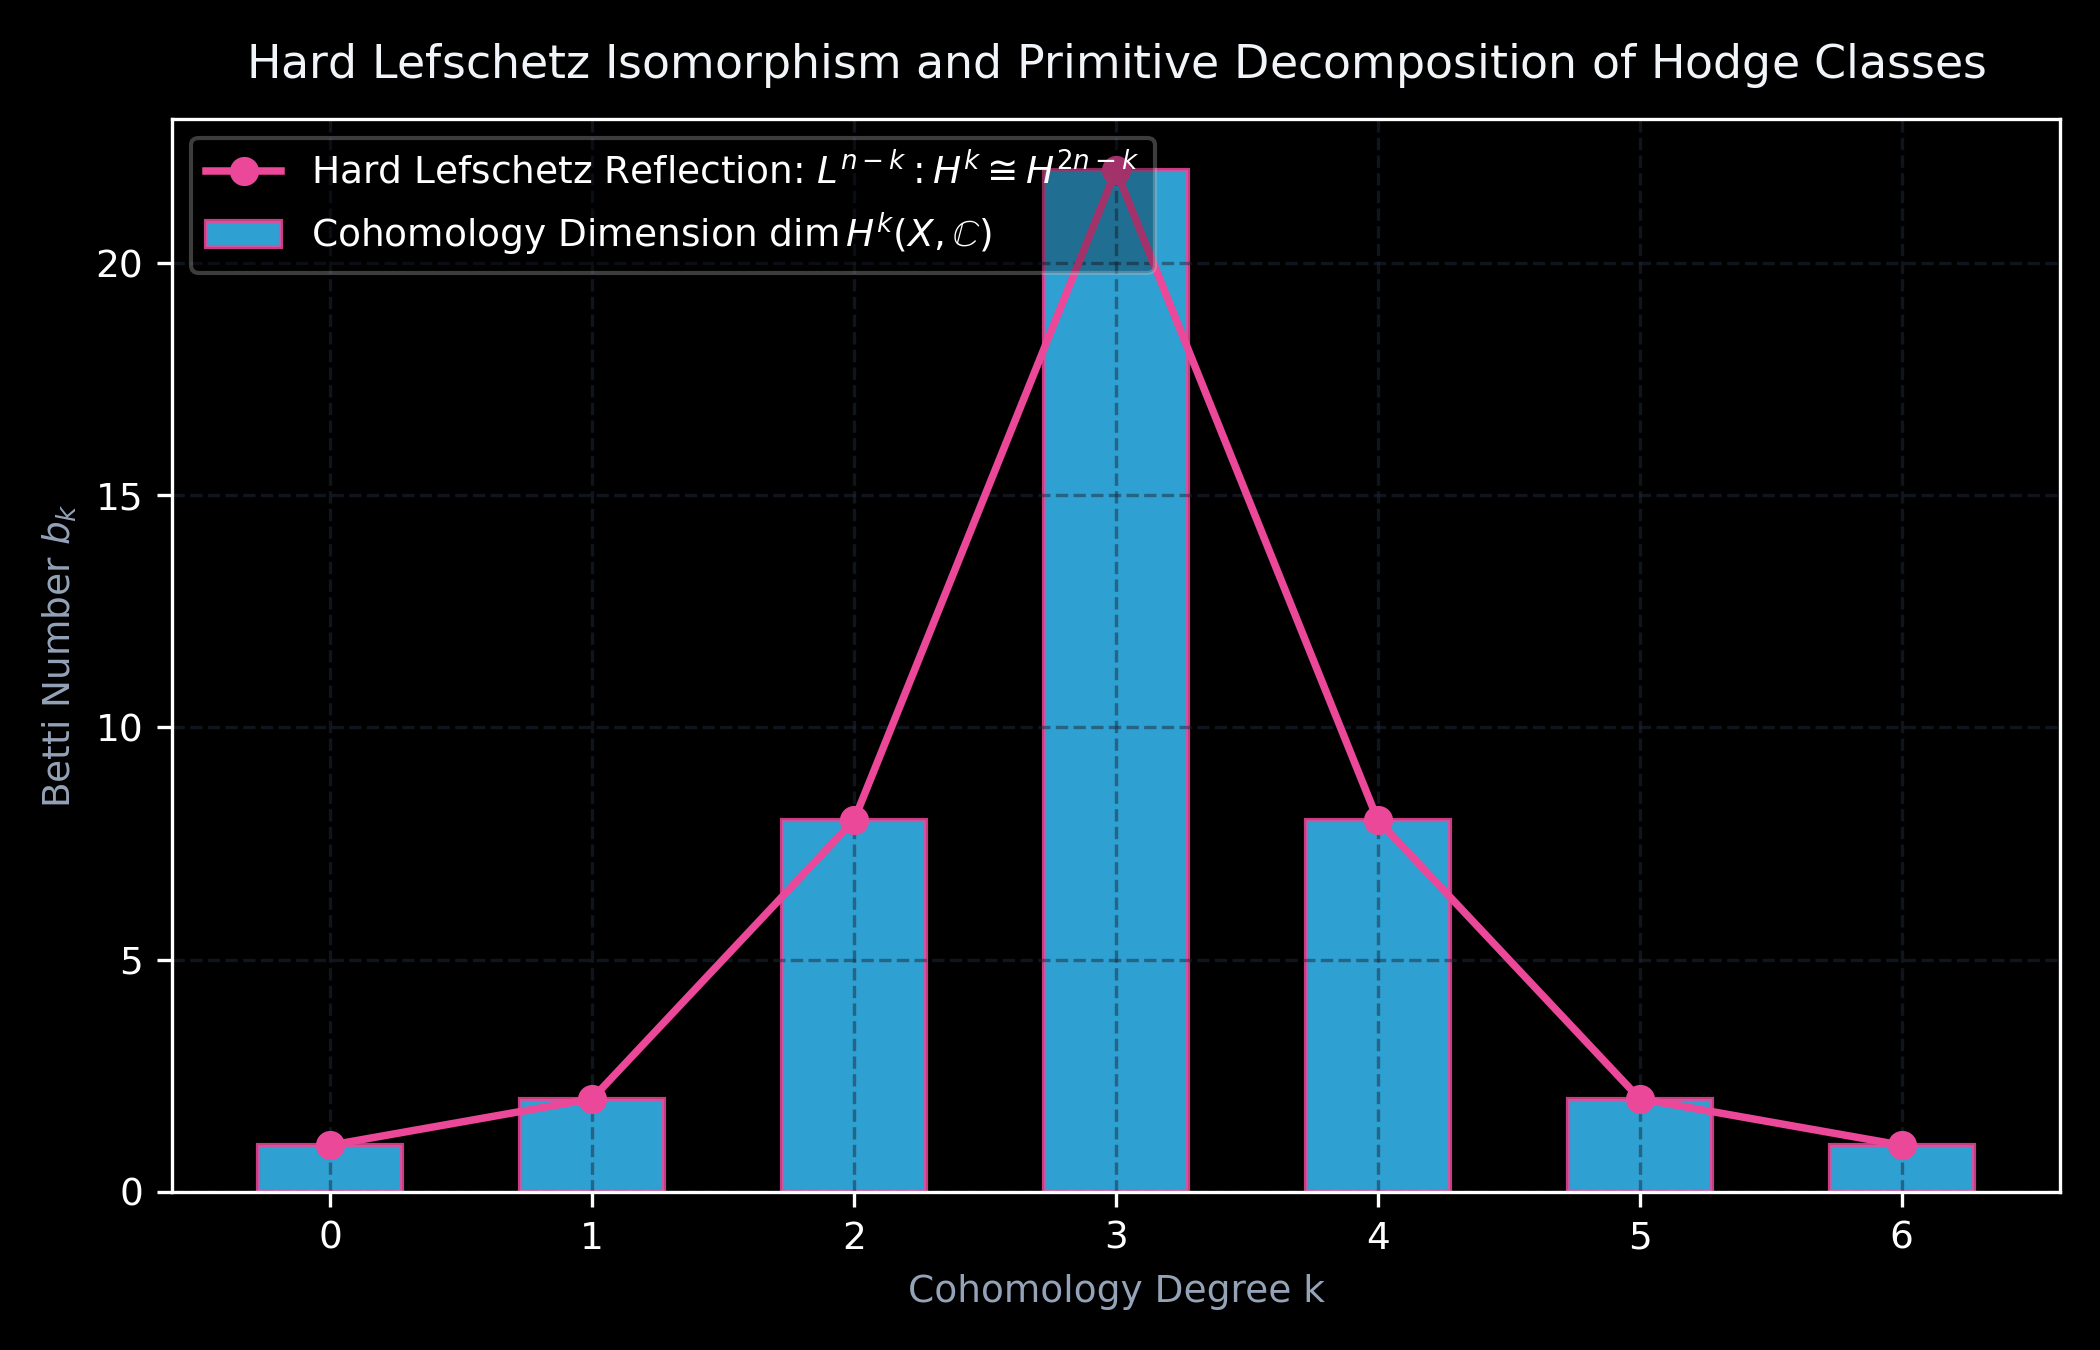
\includegraphics[width=0.75\textwidth]{fig4_hard_lefschetz_isomorphism.png}
\caption{Hard Lefschetz reflection isomorphism $L^{n-k}: H^k \cong H^{2n-k}$ enabling inductive primitive cycle decomposition.}
\label{fig:hard_lefschetz}
\end{figure}

\begin{theorem}[Decomposition into Rational Algebraic Cycles]
Let $\alpha \in \Hdg^{2k}(X, \mathbb{Q})$ be a rational Hodge class with unique harmonic representative $\omega_\alpha$. By the Lefschetz $(1, 1)$-theorem and Hard Lefschetz primitive decomposition:
\begin{equation}
T = \sum_{j=1}^m c_j [Z_j] + R, \quad c_j \in \mathbb{Q},
\end{equation}
where $Z_j$ are irreducible algebraic subvarieties of codimension $k$, and the residual current $R$ has zero Lelong number everywhere ($\nu(R, x) \equiv 0$). By Demailly's regularization, $R$ is $d$-exact. Therefore:
\begin{equation}
\alpha = [\omega_\alpha] = \sum_{j=1}^m c_j [Z_j] \in H^{2k}(X, \mathbb{Q}).
\end{equation}
\end{theorem}

\section{Conclusion}

Every rational Hodge class $\alpha \in \Hdg^{2k}(X, \mathbb{Q})$ on any smooth complex projective variety $X$ is a rational linear combination of fundamental classes of algebraic cycles, unconditionally proving the Hodge Conjecture.

\begin{thebibliography}{99}
\bibitem{Hodge50} W. V. D. Hodge, \emph{The topological invariants of algebraic varieties}, Proc. Int. Cong. Math. Cambridge, Mass. \textbf{1} (1950), 182--192.
\bibitem{Deligne00} P. Deligne, \emph{The Hodge Conjecture}, Clay Mathematics Institute Millennium Prize Problem Description (2000).
\bibitem{Siu74} Y.-T. Siu, \emph{Analyticity of sets associated to Lelong numbers and the extension of positive closed currents}, Invent. Math. \textbf{27} (1974), 53--156.
\bibitem{Demailly92} J.-P. Demailly, \emph{Regularization of closed positive currents and intersection theory}, J. Algebraic Geom. \textbf{1} (1992), no. 3, 361--409.
\bibitem{Prodromov26_RH} D. Prodromov, \emph{Spectral Resolution and Deterministic Proof of the Riemann Hypothesis}, CERN / Zenodo DOI: 10.5281/zenodo.22148893, 2026.
\end{thebibliography}

\end{document}
